Fyrr í bókinni höfum við farið yfir fjórar grunnaðgerðir sem nauðsynlegar eru til gagnagrunnsvinnslu. Við kunnum að
\begin{itemize}
 \item Búa til gagnagrunna og töflur (\verb|CREATE| skipanir, kaflar \ref{undirkafli:synidaemi-i-sql} og \ref{undirkafli:bua-til-toflu})
 \item Setja gögn inn í töflur (\verb|INSERT| skipunin, \ref{undirkafli:innsetning})
 \item Ná í gögn úr töflum (\verb|SELECT| skipunin, kaflar \ref{kafli:select} og \ref{kafli:gagnavinnslamargartoflur} eins og þeir leggja sig)
 \item Eyða töflum og öllu sem í þeim er (\verb|DROP| skipunin, kafli \ref{undirkafli:drop})
\end{itemize}
Þetta kemur okkur býsna langt. Þetta hefur hins vegar ekki leyft okkur að gera nokkrar breytingar á töflum eða þeim gögnum sem í þeim eru. Til þess þurfum við fleiri skipanir. Þær heita \verb|ALTER TABLE|, \verb|UPDATE| og \verb|DELETE|.
\section{DDL og DML}
Áður en lengra er haldið skulum við staldra við og skoða þær skipanir sem við höfum þegar kynnst.

Þessar skipanir, \verb|CREATE|, \verb|INSERT|, \verb|SELECT| og \verb|DROP| skiptast í tvo flokka. Flokkarnir kallast \emph{Data Definition Language} (DDL) og \emph{Data Manipulation Language} (DML).\footnote{Þessir flokkar hafa verið kallaðir \emph{gagnaskilgreiningarmál} og \emph{gagnameðferðarmál} á íslensku.}

DDL skipanir hafa áhrif á uppbyggingu gagnagrunnsins. Þær breyta, búa til og eyða gagnagrunnum, töflum og dálkum. \verb|CREATE| skipanir og \verb|DROP| skipunin eru DDL skipanir.

DML skipanir hafa áhrif á gögn í gagnagrunninum. Þær breyta, búa til, eyða og sýna innihald taflna. \verb|INSERT| og \verb|SELECT| eru DML skipanir.\footnote{\emph{SELECT} skipunin er örlítið sérstök hvað DML skipanir varðar, þar sem hún hefur það ekki að aðalhlutverki að breyta gögnum. Þess vegna er oft fjallað um hana sérstaklega. Hún er DML skipun engu að síður.}

Fleiri flokkar skipana eru til. Þær skipanir sem við förum yfir í þessari bók falla þó allar í þessa tvo.

\begin{marginfigure}
\caption[DDL og DML]{Yfirlit yfir þær SQL-skipanir sem við höfum séð og flokkun þeirra í DDL og DML.}
\label{mynd:inner-join}
\centering
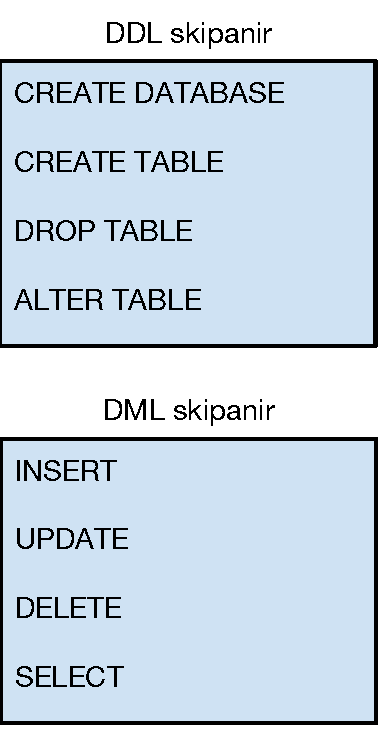
\includegraphics[width=\linewidth]{myndir/ddl-dml}
\end{marginfigure}
\section{Að breyta töflum}
Hingað til höfum við ekki farið yfir leið til að breyta töflum. Það þýðir að í hvert skipti sem villa er gerð í töflu höfum við þurft að henda töflunni ásamt öllu því sem í henni er (\verb|DROP TABLE|) og búa hana til upp á nýtt.
\section{Að breyta gögnum}
\section{Að eyða gögnum}
\section{Hreyfingar} %Transactions